\section{Experimental Setup}

\subsection{Evidence Layers}

The evidence design separates four layers: the 258-row ASR model-comparison split, selected-300 enriched high-stakes provenance outputs, a completed 300-row dual-reviewer human audit, and 900 model-level assessments per reviewer clustered within those 300 reviewed rows. Figure~\ref{fig:evidence_ladder} summarizes the design.

\begin{figure}[htbp]
\centering
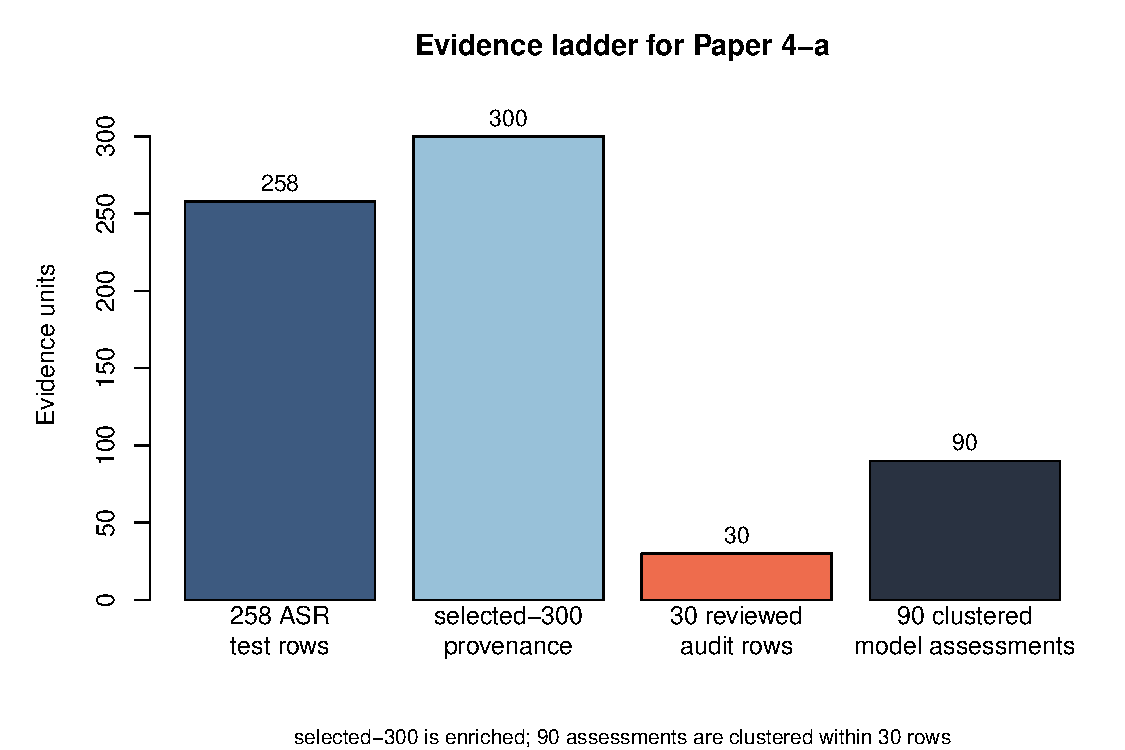
\includegraphics[width=.9\linewidth]{figures/fig2_evidence_ladder.pdf}
\caption{Evidence ladder for Paper 4-a. The figure is generated by \artifact{paper_4a_cds_asr/r/build_fig2_evidence_ladder.R} from aggregate evidence counts and the manuscript evidence boundary.}
\label{fig:evidence_ladder}
\end{figure}

The 258-row split provides ASR model-comparison context. The selected-300 layer is an enriched high-stakes audit surface and is not prevalence-preserving. The reviewed evidence layer consists of 300 rows per reviewer and 900 clustered model-level assessments per reviewer. The outcome label is human-reviewed decision change. Two reviewers completed the same selected-300 surface; Cohen's kappa is 0.849970 for decision-change labels, 1.000000 for semantic-risk labels, 0.851426 for expected safe action, and 0.934274 for annotation confidence. Reviewer agreement is treated as a validation layer over the same audit surface, while reviewer-specific labels are preserved separately for CEIS ablation rather than collapsed into an inferred adjudication.

\subsection{Baselines And Outcome}

The predictor comparison evaluates WER, CER, SRES, and CEIS against human-reviewed decision-change labels. WER and CER represent transcript-centered evidence, SRES represents semantic-risk evidence, and CEIS represents counterfactual decision-stability evidence.

\subsection{Uncertainty And Sensitivity}

Row-clustered uncertainty is reported from \artifact{70_experiments/runs/janus_300_high_stakes_human_audit_selection_2026_05_25/human_audit_predictor_clustered_ci.tsv}. Leave-one-row-out sensitivity is recorded in \artifact{70_experiments/runs/janus_300_high_stakes_human_audit_selection_2026_05_25/human_audit_predictor_leave_one_row_out.tsv}. Recovery-policy uncertainty and sensitivity are recorded in the corresponding aggregate recovery artifacts.

\subsection{CEIS Ablation Design}

The expanded dual-reviewer surface is used for an aggregate-only CEIS ablation. The variants are full CEIS, CEIS without atom weights, CEIS without plausibility, binary atom triggering, and top-3 mean aggregation over full CEIS components. The ablation isolates the mechanism that CDS-ASR contributes: decision-changing risk-atom instability under plausible alternatives. All ablation outputs are reviewer-separated aggregate summaries and exclude raw audio, transcripts, row identifiers, hypotheses, reviewer notes, and transcript-bearing merged sheets.
